\documentclass[a4paper]{book}
\usepackage[czech]{babel}
\usepackage[IL2]{fontenc}
\usepackage[utf8]{inputenc}
\usepackage{pstricks}
\usepackage{amsmath, amssymb}
\usepackage{graphicx}
\usepackage{pdfpages}
\usepackage{mathrsfs}

\usepackage{fancyhdr}
\pagestyle{fancy}
\fancyhead{}
\fancyhead[LE,RO]{\thepage}
\fancyhead[RE]{\leftmark}
\fancyhead[LO]{\rightmark}

%\includeonly{wool_chap1}

\setlength{\unitlength}{1.0mm}
\sloppy

\begin{document}

\newtheorem{definition}{Definice}[chapter]
\newtheorem{theorem}{Věta}[chapter]
\newtheorem{proof}{Důkaz}[chapter]
\newtheorem{example}{Příklad}[chapter]
\newtheorem{corollary}{Tvrzení}[chapter]
\newtheorem{assumption}{Předpoklad}[chapter]

\hyphenation{prav-dě-po-dob-nost prav-dě-po-dob-nost-ní} 

\title{Bayesiánská statistika}
\author{Ben Lambert}
\maketitle

\tableofcontents

\chapter{Úvod do logistického regresního modelu}

\section{Úvod}

V případě jednorozměrného lineárního regresního modelu předpokládáme, že střední hodnotu závislé veličiny $Y$ podmíněnou hodnotou $x$ lze vyjádřit jako
\begin{equation}
E(Y | x) = \beta_0 + \beta_1 x,
\end{equation}
kde $E(Y | x)$ může nabývat libovolné hodnoty z intervalu $(-\infty, \infty)$.

V případě logistického regresního modelu má závislá veličina binární charakter, tj. může nabývat pouze dvou hodnot. Její střední hodnota tak omezena na interval $[0, 1]$. To je také patrné z obrázku 1.1, který ilustruje závislost mezi věkem pacienta a ischemickou chorobou srdeční. Z grafu, který má tvar písmene S, je patrné, že se střední hodnota vypočtena pro jednotlivé věkové kohorty postupně blíží jedné. Graf tak můžeme chápat ve smyslu kumulativní pravděpodobnostní funkce náhodné veličiny.

\begin{figure}[htp]
\centering
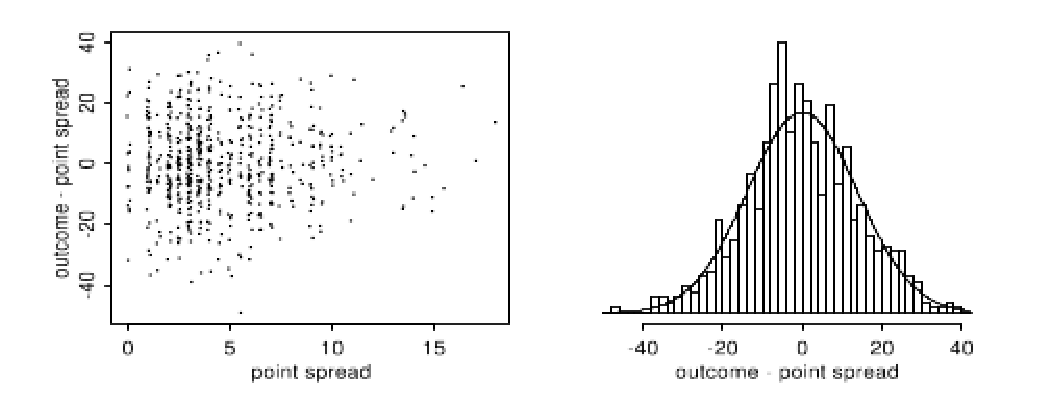
\includegraphics[scale = 0.35]{pictures/fig_1_2.eps}
\caption{Vztah mezi výskytem ischemické poruchy srdeční a věkem pacienta}
\label{fig_1_2}
\end{figure}

V následujícím textu budeme výraz $\pi(x) = E(Y | x)$ používat pro označení střední hodnoty závislé veličiny $Y$ podmíněné hodnotu $x$ pro jednorozměrný logistický regresní model, kde
\begin{equation}
\pi(x) = \frac{e^{\beta_0 + \beta_1 x}}{1 + e^{\beta_0 + \beta_1 x}}.
\end{equation}
Tuto transformaci, která je klíčová pro studium logistického regresního modelu, nazýváme logit transformací a lze ji snadno upravit do tvaru
\begin{equation}
g(x) = \ln \Big[\frac{\pi(x)}{1 - \pi(x)} \Big] = \beta_0 + \beta_1 x.
\end{equation}
Funkce $g(x)$, kterou nazýváme logit funkcí, může nabývat hodnot z intervalu $(-\infty, \infty)$.

Hodnotu závislé veličiny $y$ pro danou hodnotu $x$ můžeme vyjádřit jako $y = \pi(x) + \varepsilon$, kde $\varepsilon$ nabývá dvou stavů. Pokud $y = 1$, pak $\varepsilon = 1 -\pi(x)$ s pravděpodobností $\pi(x)$; pokud $y = 0$, pak $\varepsilon = -\pi(x)$ s pravděpodobností $1 - \pi(x)$.\footnote{Pokud $Y$ nabývá hodnot 0 popř. 1, lze $\pi(x) = E(Y | x)$ interpretovat ve smyslu pravděpodobnosti, s jakou $Y$ nabývá pro dané $x$ hodnoty 1. Pravděpodobnost, s jakou $Y$ nabývá pro dané $x$ hodnoty 0, je pak $1 - \pi(x)$.} Chyba $\varepsilon$ tak sleduje binomické rozdělení s nulovou střední hodnotou a rozptylem $\pi(x)[1 - \pi(x)]$. To je další ze zásadních rozdílů oproti lineárnímu regresnímu modelu, ve kterém chyba $\varepsilon$ sleduje normální rozdělení.

\section{Kalibrace logistického regresního modelu}

Základní metodou odhadu parametrů lineárního regresního modelu je metoda nejmenších čtverců. Podstatou této metody je volba takových hodnot parametrů $\beta_0$ a $\beta_1$, které minimalizují součet kvadrátu odchylek pozorovaných a predikovaných hodnot závislé veličiny $Y$. Tuto metodu však není v případě logistického regresního modelu možné použít.

Obecnější metodou odhadu parametrů je tzv. metoda maximální věrohodnosti, která odhadne hodnoty parametrů tak, aby výsledný model s maximální možnou pravděpodobností replikoval pozorovaná data. Za tímto účelem je třeba definovat tzv. funkci maximální věrohodnosti, která vyjadřuje pravděpodobnost výskytu pozorovaných dat v kontextu uvažovaného modelu jako funkci jeho parametrů.

Uvažujme jednorozměrný logistický regresní model a obecný pár $(x_i, y_i)$. Pokud $y_i = 1$, je kontribuce páru $(x_i, y_i)$ do funkce maximální věrohodnosti rovna $\pi(x)$. Pokud $y_i = 0$, je kontribuce páru $(x_i, y_i)$ do funkce maximální věrohodnosti rovna $1 - \pi(x)$. Tyto dva stavy lze zkombinovat do podoby
\begin{equation}
\pi(x_i)^{y_i}[1 - \pi(x_i)]^{1 - y_i}.
\end{equation}
Pokud předpokládáme, že jednotlivá pozorování představovaná páry $(x_i, y_i)$ jsou vzájemně nezávislá, lze funkci maximální věrohodnosti vyjádřit jako
\begin{equation}
l(\pmb{\beta}) = \prod_{i = 1}^n \pi(x_i)^{y_i}[1 - \pi(x_i)^{1 - y_i}].
\end{equation}
Z matematického a numerického hlediska je však snadnější pracovat s logaritmem funkce maximální věrohodnosti
\begin{equation}
L(\pmb{\beta}) = \ln[l(\pmb{\beta})] = \sum_{i = 1}^n \Big(y_i \ln[\pi(x_i) + (1 - y_i) \ln[1 - \pi(x_i)] \Big),
\end{equation}
kde $\pi(x_i) = \frac{e^{\beta_0 + \beta_1 x_i}}{1 + e^{\beta_0 + \beta_1 x_i}}$. Abychom nalezli hodnotu $\pmb{\beta}$, která maximalizuje $L(\pmb{\beta})$, je třeba nejprve derivovat $L(\pmb{\beta})$ dle $\beta_0$ a $\beta_1$ a tyto derivace položit rovny nule. Výsledné rovnice, které nazýváme rovnicemi maximální věrohodnosti, mají podobu
\begin{equation}
\sum_{i = 1}^n [y_i - \pi(x_i)] = 0
\end{equation}
a
\begin{equation}
\sum_{i = 1}^n x_i [y_i - \pi(x_i)] = 0.
\end{equation}
Rovnice maximální věrohodnosti jsou nelineární v parametrech $\beta_0$ a $\beta_1$, a proto je třeba je řešit iteračně pomocí optimalizační metody. Hodnotu $\pmb{\beta}$, která je řešením výše uvedených rovnic, značíme $\hat{\pmb{\beta}}$ a nazýváme ji odhadem maximální věrohodnosti. Podobně je $\hat{\pi}(x_i)$ odhadem maximální věrohodnosti pro $\pi(x_i)$, a platí
\begin{equation}
\hat{\pi}(x_i) = \frac{e^{\hat{\beta}_0 + \hat{\beta}_1 x_i}}{1 + e^{\hat{\beta}_0 + \hat{\beta}_1 x_i}}.
\end{equation}
Odhadnutá logit funkce pak má tvar
\begin{equation}
\hat{g}(x_i) = \hat{\beta}_0 + \hat{\beta}_1 x_i.
\end{equation}

Rovnici (1.7) lze také vyjádřit ve tvaru
\begin{equation}
\sum_{i = 1}^n y_i = \sum_{i = 1}^n \hat{\pi}(x_i),
\end{equation}
což lze interpretovat tak, že součet pozorovaných hodnot veličiny $y$ je roven součtu predikovaných hodnot.

\section{Testy významnosti odhadnutých parametrů}

\subsection{Věrohodnostní poměrový test}

Při posuzování statistické významnosti odhadnutého parametru porovnáváme pozorované hodnoty s predikovanými hodnotami získaných na základě dvou logistických regresních modelů, z nichž jeden zahrnuje zkoumanou veličinu a druhý nikoliv. Samotné porovnání modelů je pak založené na porovnání logaritmů jejich funkce maximální věrohodnosti. Pro lepší pochopení principu je užitečné o pozorovaných hodnotách přemýšlet jako o hodnotách predikovaných tzv. saturovaným model. Saturovaný logistický regresní model je takový model, který obsahuje tolik parametrů kolik je pozorovaných párů $(x_i, y_i)$.\footnote{Jednoduchým příkladem saturovaného modelu je kalibrace jednorozměrného lineárního regresního modelu na dvou pozorováních.} Porovnání pozorovaných a predikovaných hodnot je pak založeno na statistice
\begin{equation}
D = -2 \ln \Big[\frac{\textit{hodnota funkce maximální věrohodnosti kalibrovaného modelu}}{\textit{hodnota funkce maximální věrohodnosti saturovaného modelu}}\Big],
\end{equation}
kterou nazýváme věrohodnostním poměrem (likelihood ratio) a test na ní založený pak věrohodnostním poměrovým testem (likelihood ratio test). S využitím (1.6), (1.12) a skutečnosti, že pro hodnotu věrohodnostní funkce saturovaného modelu platí
\begin{equation}
l(\textit{saturovaný model}) = \prod_{i = 1}^n y_i^{y_i}(1 - y_i)^{1 - y_i},
\end{equation}
lze statistiku $D$ vyjádřit jako
\begin{equation}
D = -2 \sum_{i = 1}^n \Big[u_i \ln\Big( \frac{\hat{\pi}_i}{y_i} \Big) + (1 - y_i) \ln \Big( \frac{1 - \hat{\pi}_i}{1 - y_i} \Big) \Big],
\end{equation}
kde $\hat{\pi}_i = \hat{\pi}(x_i)$. Pokud si dále uvědomíme, že hodnota věrohodnostní funkce saturovaného modelu je vždy rovna jedné\footnote{Toto tvrzení lze snadno ověřit dosazením $y_i = 1$ a $y_i = 0$ do (1.13).}, lze (1.12) zjednodušit do podoby
\begin{equation}
D = -2 \ln (\textit{hodnota funkce maximální věrohodnosti kalibrovaného modelu}).
\end{equation}

Pro účely zhodnocení významnosti nezávislé veličiny pak porovnáváme věrohodnostní poměr $D$ pro model s a bez uvažované veličiny, tj.
\begin{multline}
G = D(\textit{hodnota funkce maximální věrohodnosti bez uvažované veličiny}) - \\
D(\textit{hodnota funkce maximální věrohodnosti s uvažovanou veličinou}),
\end{multline}
což lze dále upravit na
\begin{equation}
G = -2 \ln \left[\frac{\textit{hodnota funkce maximální věrohodnosti bez uvažované veličiny}}{\textit{hodnota funkce maximální věrohodnosti s uvažovanou veličinou}}\right].
\end{equation}
Lze snadno dokázat, že v případě modelu, který zahrnuje pouze parametr $\beta_0$, je odhad tohoto parametru roven $\ln(n_1 / n_0)$, kde $n_1 = \sum_{i = 1}^n y_i$ a $n_0 = \sum_{i = 1}^n (1 - y_i)$ a predikovaná hodnota má charakter konstanty $n_1 / n$. V tomto případě pak pro námi uvažovaný jednorozměrný logistický regresní model platí
\begin{equation}
G = -2 \ln \left[\frac{\Big(\frac{n_1}{n}\Big)^{n_1}\Big(\frac{n_0}{n}\Big)^{n_0}}{\prod_{i = 1}^n \hat{\pi}_i (1 - \hat{\pi}_i)^{1 - y_i}}\right].
\end{equation}

Při platné nulové hypotéze $H_0: \beta_1 = 0$ sleduje $G$ chi-kvadrát rozdělení s jedním stupněm volnosti.

\subsection{Waldův test}

Alternativou k věrohodnostnímu poměrovému testu je Waldův test, který poměřuje hodnotu odhadnutého parametru $\hat{\beta}_1$ k jeho směrodatné odchylce. Výsledný poměr
\begin{equation}
W = \frac{\hat{\beta}_1}{\widehat{se}(\hat{\beta}_1)}
\end{equation}
při platnosti nulové hypotézy $H_0: \beta_1 = 0$ sleduje standardní normální rozdělení. Nevýhodou Waldova testu bohužel je, že často nezamítne nulovou hypotézu ani v případě, kdy je odhadnutý parametr významný. Proto je vhodnější používat věrohodnostní poměrový test.

\subsection{Skóre test}

Dalším možným testem významnosti parametru je tzv. skóre test, jehož hlavní výhodou je nižší výpočetní náročnost. Test je založen na teorii pravděpodobnostního rozdělení derivace logaritmu věrohodnostní funkce. Konkrétně v případě jednorozměrného logistického regresního modelu je test založen na znalosti pravděpodobnostního rozdělení derivace (1.8) podmíněné derivací (1.7). Test používá hodnotu rovnice (1.8) vypočtenou s pomocí $\beta_0 = \ln(n_1 / n_0)$ a $\beta_1 = 0$. Jak již bylo zmíněno dříve, platí pro tento případ $\hat{\pi} = n_1 / n = \overline{y}$. Dále lze dokázat, že odhadovaný rozptyl je $\overline{y}(1 - \overline{y}) \sum (x_i - \overline{x})^2$. To vede ke statistice
\begin{equation}
ST = \frac{\sum_{i = 1}^n x_i (y_i - \overline{y})}{\sqrt{\overline{y}(1 - \overline{y}) \sum_{i = 1}^n (x_i - \overline{x})^2}},
\end{equation}
která opět sleduje standardizované normální rozdělení. Opět nicméně platí, že věrohodnostní poměrový test je preferovaný před skóre testem.

\section{Intervaly spolehlivosti}

Intervaly spolehlivosti odhadnutých parametrů jsou založeny na Waldově testu a mají tvar
\begin{equation}
\hat{\beta}_i \pm z_{1 - \alpha / 2} \widehat{se}(\hat{\beta}_i).
\end{equation}
Takto definované intervaly spolehlivosti lze použít nejen pro $\beta_1$ ale také pro konstantní člen modelu $\beta_0$.

Podobným způsobem lze také odhadnout intervaly spolehlivosti pro logit funkci. Střední hodnota logit funkce je definována jako
\begin{equation}
\hat{g}(x) = \hat{\beta}_0 + \hat{\beta}_1 x
\end{equation}
a její rozptyl v případě jednorozměrného logistického regresního modelu jako
\begin{equation}
\widehat{var}[g(x)] = \widehat{var}(\hat{\beta}_0) + x^2 \widehat{var}(\hat{\beta}_1) + 2 x \widehat{cov}(\hat{\beta}_0, \hat{\beta}_1).
\end{equation}
Interval spolehlivosti logit funkce pak lze vypočíst pomocí
\begin{equation}
\hat{g}(x) \pm z_{1 - \alpha / 2}\widehat{se}[\hat{g}(x)],
\end{equation}
kde $\widehat{se}[\hat{g}(x)] = \sqrt{\widehat{var}[g(x)]}$. Protože střední hodnota $\hat{\pi}(x)$ je definována jako $\frac{e^{\hat{g}(x)}}{1 + e^{\hat{g}(x)}}$, lze interval spolehlivosti pro $\hat{\pi}(x)$ určit pomocí
\begin{equation}
\frac{e^{\hat{g}(x) \pm z_{1 - \alpha / 2} \widehat{se}[\hat{g}(x)]}}{1 + e^{\hat{g}(x) \pm z_{1 - \alpha / 2} \widehat{se}[\hat{g}(x)]}}.
\end{equation}


\end{document}
